\documentclass[stu, 12pt, letterpaper, donotrepeattitle, floatsintext, natbib]{apa7}
\usepackage[utf8]{inputenc}
\usepackage[T1]{fontenc}
\usepackage{adjustbox}
\usepackage{longtable}
\usepackage{tabularx}
\usepackage{lmodern}
\usepackage{comment}
\usepackage{marvosym}
\usepackage{graphicx}
\usepackage{float}
\usepackage[normalem]{ulem}
\usepackage[spanish]{babel}
\usepackage{multirow}
\usepackage{tabularx}
\usepackage{tabularray}
\usepackage{adjustbox}
\usepackage{geometry}
\usepackage{tikz}
\usepackage{enumitem}
\usepackage{hyperref}
\usepackage{amsmath}
\usepackage{pgfgantt}
\usepackage{apacite}
\usepackage{array}

\usetikzlibrary{shapes.geometric, arrows, positioning, fit, calc}
\selectlanguage{spanish}
\useunder{\uline}{\ul}{}
\newcommand{\myparagraph}[1]{\paragraph{#1}\mbox{}\\}

% Portada
\title{\Large Plan de Pruebas}
\author{
    Campero Morales José Antonio \\
    Campohermoso Berdeja Oscar \\
    Carrasco Cespedes Miguel Alejandro \\
    Martinez Acarapi Fabiola Alejandra \\
    Montero Garrido Diana Aneliz \\
    Zizold Sempertegui Gabriela Zulema Britta
}
\affiliation{Universidad Católica Boliviana}
\course{SIS-312: Gestión de Calidad de Sistemas}
\professor{Lic. Cecilia Alvarado Monrroy}
\duedate{\textbf{28 de octubre de 2024}}

\newcommand{\userstory}[5]{ % Change from 4 to 5 arguments
    \begin{center}
        \begin{tikzpicture}
            \node[draw, rounded corners, fill=blue!10, text width=0.9\textwidth, align=center, inner sep=10pt] {
                \textbf{#1} \\[5pt]
                \textit{Como} #2, \\[5pt]
                \textit{quiero} #3 \\[5pt]
                \textit{para} #4 \\[5pt]
                \href{#5}{Ver en GitHub} 
            };
        \end{tikzpicture}
    \end{center}
    \vspace{10pt}
}

\begin{document}
\thispagestyle{empty}

% Add the logo before the title content, avoiding extra space
\centering

\includegraphics[width=0.8\textwidth]{../imgs/logo-ucb.png} % Adjust the path to your logo image
\vspace{-5cm} % Adjust negative space if needed

\maketitle

% Índices
\newpage
\pagenumbering{roman}
% Contenido
\renewcommand\contentsname{\large Índice}
\tableofcontents
\setcounter{tocdepth}{2}
\newpage
% Fíguras
\renewcommand{\listfigurename}{\large Índice de figuras}
\listoffigures
\newpage
% Tablas
\renewcommand{\listtablename}{\large Índice de tablas}
\listoftables
\newpage

% Cuerpo
\pagenumbering{arabic}
\section{\large Introducción}

\noindent El sistema esarrollado en la materia de Análisis de Algoritmos durante el periodo 1-2024 permite probar y analizar diversos tipos de algoritmos, cada uno implementado en un editor especializado. Estos editores están diseñados para adaptarse a las características específicas de cada algoritmo, permitiendo diferentes enfoques según los requisitos: algunos permiten la creación y visualización de grafos y la generación de matrices de adyacencia, mientras que otros, como los algoritmos de ordenamiento, se centran en la manipulación y visualización de datos ordenados. Este enfoque modular facilita un análisis práctico y enfocado en las propiedades de cada tipo de algoritmo.

\noindent El \textit{editor Northwest}, uno de los editores desarrollados, está diseñado específicamente para el método de la esquina noroeste (\textit{Northwest Corner Method}), una técnica utilizada para resolver problemas de transporte y asignación de recursos. Este método ofrece una solución inicial factible al distribuir suministros y demandas de manera efectiva, lo cual facilita la posterior optimización del costo total de transporte.

\noindent La elección de este editor para el plan de pruebas responde al interés de explorar cómo este algoritmo puede generar soluciones iniciales basadas en condiciones específicas de oferta y demanda. Además, el editor Northwest permite la manipulación visual de grafos y la generación de la matriz de adyacencia, convirtiéndolo en una herramienta práctica tanto para el análisis como para la resolución de problemas de asignación. A continuación, se presenta un plan de pruebas para asegurar la funcionalidad completa y la robustez del editor Northwest.

\subsection{Alcance}

\subsubsection{Las pruebas abarcarán las siguientes áreas:}

\begin{itemize}
    \item \textbf{Creación y visualización de grafos:} Se verificará que el editor permita la creación precisa de grafos, incluyendo la adición y conexión de nodos y aristas, asegurando que los grafos generados se representen correctamente en el entorno gráfico del editor.

    \item \textbf{Guardado y carga de grafos:} Se evaluará la funcionalidad de guardado de grafos, comprobando que los datos se almacenen correctamente y que puedan ser recuperados sin pérdida de información, para permitir la continuidad del análisis y la manipulación de los grafos en futuras sesiones.

    \item \textbf{Generación de la matriz de adyacencia:} Se revisará que el editor construya de manera precisa la matriz de adyacencia a partir de los grafos creados, asegurando que refleje adecuadamente las conexiones y relaciones entre los nodos en el grafo.

    \item \textbf{Generación de la matriz de costos:} Se evaluará la construcción precisa de la matriz de costos basada en los nodos y sus conexiones, garantizando que refleje las relaciones correctas entre puntos de suministro y demanda.

    \item \textbf{Optimización:} Se verificará que el módulo de optimización sea capaz de resolver tanto problemas de maximización como de minimización, validando que los resultados sean consistentes con los objetivos definidos en el editor.

    \item \textbf{Interfaz, usabilidad y accesibilidad:} Se revisará la facilidad de uso del formulario de entrada, asegurando que los elementos interactivos sean intuitivos y que el editor responda adecuadamente a diferentes valores de entrada. Además, se realizarán pruebas de accesibilidad para garantizar que el editor cumpla con los estándares de accesibilidad definidos.
\end{itemize}

\vspace{1cm}
\subsubsection{Las pruebas no abarcarán las siguientes áreas:}

\begin{itemize}
    \item \textbf{Componentes fuera del editor:} No se evaluarán elementos externos al editor, como la manipulación de archivos de grafos creados previamente que se realiza antes de ingresar al editor, ni la descripción del algoritmo en la interfaz inicial. Incluir estas áreas implicaría evaluar funcionalidades que están fuera del alcance directo del editor.
    
    \item \textbf{Pruebas de desempeño bajo condiciones extremas de carga:} No se realizarán pruebas de estrés en esta fase del proyecto; sin embargo, estas pruebas serán consideradas para futuras iteraciones.
    
\end{itemize}

\subsection{Objetivo}

\noindent Las pruebas tienen como objetivo asegurar que el editor \textit{Northwest} cumpla con los requisitos funcionales y no funcionales establecidos, garantizando que las soluciones generadas para distintas configuraciones de oferta y demanda sean precisas y consistentes. Este proceso incluirá la verificación de la conformidad del editor con los estándares de calidad definidos por el cliente, y se centrará en:

\begin{itemize}
    \item Validar la precisión de los resultados generados en términos de optimización, asegurando que se ajusten a los objetivos de maximización o minimización.
    \item Evaluar la usabilidad y accesibilidad de la interfaz, verificando que los elementos interactivos sean intuitivos y que el editor sea accesible según los estándares de accesibilidad definidos.
    \item Detectar y documentar posibles errores y áreas de mejora, permitiendo su corrección antes de la implementación en producción, para maximizar la satisfacción del usuario final y asegurar una experiencia de usuario eficiente y libre de problemas.
\end{itemize}

\subsection{Limitaciones}

\begin{itemize}
    \item \textbf{Datos de prueba limitados:} La disponibilidad de datos de prueba representativos es limitada, lo que podría restringir la validación a configuraciones específicas de oferta y demanda, dejando fuera algunos escenarios posibles que podrían presentarse en situaciones reales.

    \item \textbf{Configuración de grafos predefinida:} Debido a que este es un problema de asignación, la configuración de grafos utilizada está previamente definida y limitada a ciertos parámetros específicos. Esto significa que el editor no se someterá a pruebas en configuraciones de grafos alternativas o personalizables, lo que podría limitar la flexibilidad de los resultados en otros escenarios de aplicación.
\end{itemize}

\subsection{Base de la Prueba}

\subsubsection{Requisitos del Sistema}
Los requisitos del sistema definen las necesidades y expectativas que el editor \textit{Northwest} debe cumplir para asegurar una funcionalidad completa y efectiva. Estos incluyen:

\begin{itemize}
    \item \textbf{Creación y visualización de grafos}: 
    El editor deberá permitir a los usuarios crear grafos, incluyendo la adición de nodos y aristas, y visualizar los grafos de forma clara e intuitiva dentro de la interfaz del editor.

    \item \textbf{Carga y descarga de grafos}: 
    El editor permitirá a los usuarios cargar grafos guardados desde su computador y descargar los grafos creados para su almacenamiento local, asegurando que la información se maneje de forma precisa y sin pérdidas.

    \item \textbf{Generación automática de la matriz de adyacencia}: 
    A partir de los grafos creados en el editor, este deberá generar automáticamente una matriz de adyacencia que refleje correctamente las conexiones entre los nodos definidos.

    \item \textbf{Generación automática de la matriz de costos}: 
    El editor deberá generar de manera automática una matriz de costos basada en los nodos y conexiones definidas por el usuario, asegurando que la información de costos esté alineada con los datos ingresados.

    \item \textbf{Manejo de oferta y demanda}: 
    El editor deberá gestionar situaciones donde la oferta y la demanda no estén balanceadas. Si es necesario, ajustará automáticamente las configuraciones para asegurar que no se produzcan errores en los cálculos de transporte.

    \item \textbf{Funcionalidades de optimización}: 
    El editor deberá ofrecer opciones que permitan al usuario seleccionar entre maximización o minimización de soluciones, proporcionando resultados válidos y ajustados a los objetivos especificados en las configuraciones de entrada.

    \item \textbf{Accesibilidad del editor}: 
    Aunque no se ha pensado en un nivel profundo de accesibilidad, se espera que el editor, como mínimo, tenga un buen contraste de colores y cumpla con un nivel básico de accesibilidad.
\end{itemize}


\subsubsection{Especificaciones Funcionales}

Estas especificaciones detallan cada función del editor \textit{Northwest} y el comportamiento esperado, proporcionando instrucciones claras para los desarrolladores:

\begin{itemize}
    \item \textbf{Creación y visualización de grafos}:
    \begin{itemize}
        \item \textbf{Función}: Permitir la creación y visualización de grafos.
        \item \textbf{Requisitos funcionales}:
            \begin{itemize}
                \item El editor deberá permitir a los usuarios definir nodos y conexiones con pesos dentro del editor.
                \item Los grafos creados deben ser visualizados de forma intuitiva en la interfaz gráfica del editor.
                \item Se notificará al usuario si hay inconsistencias en la entrada de datos para asegurar la precisión en la creación del grafo.
            \end{itemize}
        \item \textbf{Proceso}:
            \begin{itemize}
                \item Al definir nodos y conexiones, el editor mostrará visualmente el grafo en tiempo real.
                \item Cualquier cambio en los nodos o aristas reflejará una actualización inmediata en la visualización.
            \end{itemize}
    \end{itemize}

    \item \textbf{Carga y descarga de grafos}:
    \begin{itemize}
        \item \textbf{Función}: Permitir la carga de grafos desde el computador y la descarga de grafos creados en el editor.
        \item \textbf{Requisitos funcionales}:
            \begin{itemize}
                \item El editor deberá permitir al usuario cargar grafos guardados en su computador en formato JSON, para que preserve toda la información de los nodos y conexiones.
                \item El editor deberá permitir al usuario descargar los grafos creados en formato JSON, garantizando así su integridad y que se puedan volver a cargar sin pérdida de 
                \item El editor deberá notificar al usuario sobre el estado de carga y descarga, indicando si estas operaciones se realizaron con éxito o si se presentaron problemas.
            \end{itemize}
        \item \textbf{Proceso}:
            \begin{itemize}
                \item El usuario podrá cargar grafos guardados en su computador en cualquier momento y descargará grafos generados para su almacenamiento local.
            \end{itemize}
    \end{itemize}


    \item \textbf{Generación de la matriz de adyacencia}:
    \begin{itemize}
        \item \textbf{Función}: Generación automática de la matriz de adyacencia a partir del grafo.
        \item \textbf{Requisitos funcionales}:
            \begin{itemize}
                \item El editor deberá calcular automáticamente la matriz de adyacencia que refleje las conexiones entre los nodos del grafo.
                \item El editor deberá permitir al usuario visualizar la matriz de adyacencia generada.
            \end{itemize}
        \item \textbf{Proceso}:
            \begin{itemize}
                \item Una vez creado el grafo, el editor generará automáticamente la matriz de adyacencia y permitirá su visualización al usuario.
                \item La matriz de adyacencia deberá reflejar correctamente las relaciones entre los nodos y las conexiones.
            \end{itemize}
    \end{itemize}

    \item \textbf{Generación de la matriz de costos}:
    \begin{itemize}
        \item \textbf{Función}: Generación automática de la matriz de costos basada en los pesos de las conexiones.
        \item \textbf{Requisitos funcionales}:
            \begin{itemize}
                \item El editor deberá permitir al usuario definir nodos y conexiones con pesos.
                \item El editor calculará la matriz de costos utilizando los valores de los pesos de las conexiones.
                \item La matriz de costos deberá reflejar correctamente las relaciones entre los puntos de suministro y demanda.
            \end{itemize}
        \item \textbf{Proceso}:
            \begin{itemize}
                \item Al definir nodos y conexiones, el editor generará automáticamente la matriz de costos.
            \end{itemize}
    \end{itemize}

    \item \textbf{Ajuste de oferta y demanda}:
    \begin{itemize}
        \item \textbf{Función}: Ajuste automático cuando la oferta y demanda no coinciden.
        \item \textbf{Requisitos funcionales}:
            \begin{itemize}
                \item El editor deberá añadir un nodo ficticio cuando los valores de oferta y demanda no estén balanceados.
                \item El editor deberá ajustar la matriz de costos para reflejar el nodo ficticio y balancear la matriz.
                \item El usuario deberá ser notificado sobre el ajuste realizado y cómo afecta a la solución.
            \end{itemize}
        \item \textbf{Proceso}:
            \begin{itemize}
                \item Si hay desequilibrio entre oferta y demanda, se añadirá un nodo ficticio para balancear la matriz.
                \item La matriz de costos se ajustará automáticamente para reflejar el nodo ficticio y los cambios en la solución.
            \end{itemize}
    \end{itemize}
    
    \item \textbf{Optimización}:
    \begin{itemize}
        \item \textbf{Función}: Cálculo de soluciones optimizadas.
        \item \textbf{Requisitos funcionales}:
            \begin{itemize}
                \item El editor permitirá al usuario elegir entre criterios de maximización y minimización.
                \item El editor calculará la solución óptima basada en el criterio seleccionado.
                \item El editor mostrará la solución optimizada al usuario de forma clara y comprensible.
            \end{itemize}
        \item \textbf{Proceso}:
            \begin{itemize}
                \item El usuario seleccionará un criterio de optimización y el editor calculará la solución optimizada.
                \item La solución se mostrará al usuario de forma clara y comprensible, en una tabla.
            \end{itemize}
    \end{itemize}
\end{itemize}


\subsubsection{Historias de Usuario}

Las siguientes historias de usuario documentan los requisitos específicos y su relación con las especificaciones funcionales descritas en la sección de \textbf{Especificaciones Funcionales}. Cada historia de usuario puede consultarse en el \textit{Anexo A}, donde se detallan los parámetros y contexto para cada funcionalidad. Estas historias serán fundamentales para la creación de casos de prueba

\begin{description}

    \item[HU006-GraphEditor] \hfill \\
    Describe los requisitos para que el usuario pueda agregar nodos y aristas, y modificar sus valores dentro del editor gráfico. Esta historia de usuario se relaciona directamente con la especificación funcional de \textbf{Creación y visualización de grafos} ya que define cómo debe construirse y modificarse el grafo en la interfaz gráfica del editor. \textit{\hyperref[tab:HU006-GraphEditor]{Ver Anexo HU006-GraphEditor}}

    \item[HU007-AdjacentMatrix] \hfill \\
    Documenta la necesidad del usuario de obtener la matriz de adyacencia del grafo generado. Esta historia respalda la especificación funcional de \textbf{Generación de la matriz de adyacencia} y establece que el sistema debe mostrar las conexiones entre nodos en un formato estructurado. \textit{\hyperref[tab:HU007-AdjacentMatrix]{Ver Anexo HU007-AdjacentMatrix}}

    \item[HU008-FileManagement] \hfill \\
    Define los requisitos para guardar el grafo en formato JSON y cargarlo posteriormente con todos sus elementos intactos. Esta historia está vinculada a la especificación funcional de \textbf{Carga y descarga de grafos}, asegurando que el usuario pueda conservar su trabajo sin pérdida de información. \textit{\hyperref[tab:HU008-FileManagement]{Ver Anexo HU008-FileManagement}}

    \item[HU009-NorthWest-01] \hfill \\
    Documenta los requisitos para la generación automática de la matriz de costos con base en los pesos de las conexiones definidas por el usuario. Relacionada con la especificación funcional de \textbf{Generación de la matriz de costos}, esta historia establece cómo se debe reflejar la estructura de costos entre puntos de suministro y demanda. \textit{\hyperref[tab:HU009-NorthWest-01]{Ver Anexo HU009-NorthWest-01}}

    \item[HU010-NorthWest-02] \hfill \\
    Detalla la necesidad de manejar desequilibrios entre oferta y demanda, añadiendo un nodo ficticio cuando sea necesario. Este requisito se relaciona con la especificación funcional de \textbf{Ajuste de oferta y demanda}, describiendo cómo el sistema debe ajustarse automáticamente para mantener el equilibrio en la matriz de costos. \textit{\hyperref[tab:HU010-NorthWest-02]{Ver Anexo HU010-NorthWest-02}}

    \item[HU011-NorthWest-03] \hfill \\
    Especifica la capacidad del sistema para generar soluciones válidas según diversas configuraciones y criterios de optimización. Esta historia se relaciona con la especificación funcional de \textbf{Optimización}, asegurando que los resultados sean precisos y que el usuario pueda seleccionar el criterio de optimización deseado. \textit{\hyperref[tab:HU011-NorthWest-03]{Ver Anexo HU011-NorthWest-03}}

\end{description}

\subsubsection{Diagramas de Flujo de Datos y Procesos}

Los diagramas de flujo de datos y procesos en el \hyperref[tab:flowchart]{Anexo B: Diagrama de Flujo de Proceso para el Editor Northwest} y el \hyperref[tab:dataflow]{Anexo B: Diagrama de Flujo de Datos para el Editor Northwest} resultan útiles para entender el funcionamiento del editor Northwest, y serán de gran utilidad para el Plan de Pruebas. Estos muestran cómo se gestiona la entrada de datos del grafo, la definición de datos y las posibles acciones, como la generación de matrices de adyacencia y costos, así como el guardado de datos en JSON. También ilustran el proceso de optimización, que culmina en una solución optimizada. Estos diagramas pueden ser de gran ayuda para visualizar los pasos y decisiones claves en la manipulación de grafos dentro del editor.

\subsubsection{Arquitectura del Software}
Esta arquitectura del sistema es fundamental para identificar los objetos de prueba dentro del plan de pruebas. La configuración actual consiste en una mezcla de arquitectura monolítica con microservicios debido al uso de múltiples servicios externos. Para ver el diagrama de arquitectura detallado, consulte el \hyperref[fig:architecture]{Anexo B: Diagrama de Arquitectura del Sistema}.

La interfaz de usuario, desarrollada en Vue.js, se encarga de descargar y cargar el grafo, tareas independientes del almacenamiento en MinIO. FastAPI maneja las solicitudes del modelo de transporte a través de la API `http://localhost:8000/transportation/`, a la cual se le envía el grafo, la oferta, la demanda, y el criterio de optimización (minimizar o maximizar), y devuelve la solución óptima. Por otra parte, el endpoint `http://localhost:8081/graph/adjMatrix` en el servicio Spring genera la matriz de adyacencia necesaria para las operaciones de grafo.

\section{\large Supuestos y Limitaciones del Proyecto de Prueba}

\begin{itemize}
    \item \textbf{Vigencia de autenticación:} Se supone que los tokens de autenticación utilizados en el sistema tienen una duración de 30 minutos. Esto implica que, para mantener la validez de estos tokens y no interrumpir el proceso de pruebas, las pruebas deben contemplar este límite de tiempo.
    
    \item \textbf{Servicios auxiliares no utilizados:} Existen ciertos servicios auxiliares configurados que no se utilizarán directamente en este entorno de pruebas. Por lo tanto, se asumirán levantados para mantener la estructura de la arquitectura, pero no serán considerados en las pruebas.
    
    \item \textbf{Creación de datos simulados (mocks):} Es probable que para algunas pruebas se requiera la creación de datos simulados, especialmente para el proceso de optimización y generación de matrices. Se asumirán estos datos como representativos para validar el funcionamiento de los algoritmos.

    \item \textbf{Limitaciones en los datos de prueba:} La disponibilidad de datos de prueba se limita a ciertas configuraciones de oferta y demanda representativas, lo cual podría restringir la validación del sistema a escenarios específicos. Esto significa que podrían quedar fuera algunos casos extremos o poco comunes.
    
    \item \textbf{Configuración de grafos predefinida:} Debido a la naturaleza del problema de asignación, la configuración de grafos que se probará estará predefinida en el sistema, limitando la flexibilidad para probar variaciones personalizadas de grafos. Esto es una limitación para analizar escenarios alternativos.
\end{itemize}

\section{\large Partes Interesadas}

\subsection{Equipo de Desarrollo} 
El equipo de desarrolladores responsables de la implementación de todo el sistema está compuesto por:
    \begin{itemize}
        \item Oscar Campohermoso Berdeja
        \item Miguel Alejandro Carrasco Céspedes
        \item Oscar Menacho Silva
        \item Sebastián Orias Bellido
    \end{itemize}

\subsection{Equipo de Pruebas (QA)} 
El equipo de pruebas está liderado por Oscar Campohermoso Berdeja, quien asume tanto el \textit{Rol de gestión de pruebas} como el \textit{Rol de pruebas}. Actualmente, está encargado de planificar, diseñar y ejecutar pruebas para asegurar el funcionamiento correcto del sistema. Sus tareas también incluyen la documentación de los resultados y la identificación de problemas o áreas de mejora.

\subsection{Usuarios Finales} 
Los estudiantes y docentes de la materia de Análisis de Algoritmos utilizan el editor \textit{Northwest} como herramienta pedagógica. Su interés principal radica en la precisión de los resultados de optimización y en la facilidad de uso de la interfaz, aspectos clave para una experiencia de aprendizaje efectiva.

\subsection{Stakeholders Académicos} 
El profesor de la materia, Ing. Yamil Cárdenas, quien supervisa el uso del editor en el contexto académico. Su interés es que el editor cumpla con los objetivos educativos, permitiendo a los estudiantes experimentar con algoritmos de manera confiable e intuitiva.

\section{\large Comunicación}

\noindent La comunicación de los resultados y hallazgos se llevará a cabo mediante un informe de resultados que incluirá todos los aspectos evaluados y observaciones relevantes.

\begin{itemize}
    \item \textbf{Informe final de resultados:} Los resultados se presentarán formalmente en un informe final, que abarcará:
    \begin{itemize}
        \item Un análisis completo de los defectos encontrados en cada etapa de la prueba, categorizados según el tipo de prueba realizada: funcionalidad, usabilidad y accesibilidad.
        \item Métricas de desempeño de las pruebas, tales como la cantidad de casos de prueba ejecutados y la tasa de éxito, con visualizaciones para facilitar su interpretación.
        \item Referencia directa a los Test Cases en anexos, que servirán como soporte detallado y herramienta de comunicación, permitiendo una revisión exhaustiva de cada caso probado.
    \end{itemize}

    \item \textbf{Reporte de defectos:} Los defectos identificados serán documentados en reportes específicos según el tipo de prueba:
    \begin{itemize}
        \item \textbf{Reporte de defectos de pruebas funcionales}: Detallado en anexos, cubriendo hallazgos en la funcionalidad del editor Northwest (\hyperref[tab:reporte_defectos]{ver en Anexos}).
        \item \textbf{Reporte de defectos de pruebas de accesibilidad}: Incluirá observaciones sobre la accesibilidad en la interfaz (\hyperref[tab:reporte_accesibilidad]{ver en Anexos}).
        \item \textbf{Reporte de defectos de usabilidad}: Basado en heurísticas de Nielsen, con observaciones sobre la experiencia de usuario (\hyperref[tab:reporte_usabilidad]{ver en Anexos}).
    \end{itemize}

    
    \item \textbf{Dashboard de métricas:} Como complemento visual, el informe incluirá un dashboard sencillo que resuma los siguientes indicadores:
    \begin{itemize}
        \item Número total de Test Cases ejecutados.
        \item Proporción de casos exitosos, presentados mediante gráficos circulares para facilitar su interpretación.
    \end{itemize}
\end{itemize}

\section{\large Registro de Riesgos}

\noindent A continuación, se presenta un registro de riesgos que abarca tanto los riesgos del proyecto como del producto. Estos riesgos podrían impactar en la ejecución, calidad y resultados esperados del editor \textit{Northwest}. 

\subsection{Riesgos de Proyecto}
Estos riesgos están asociados a factores de gestión y control del proyecto, lo que incluye problemas organizacionales, limitaciones de recursos y cuestiones técnicas.

\begin{itemize}
    \item \textbf{Cuestiones de organización:}
    \begin{itemize}
        \item \textbf{Disponibilidad limitada del equipo de desarrollo:} Dos de los cuatro desarrolladores asignados al proyecto no estarán disponibles para resolver bugs, lo cual podría retrasar la corrección de errores y afectar los plazos de entrega.
        \item \textbf{Falta de experiencia en áreas clave:} La ausencia de personal especializado en rendimiento y accesibilidad limita la capacidad del equipo para realizar pruebas profundas en estas áreas, lo que podría afectar la calidad final del producto en términos de usabilidad y desempeño.
    \end{itemize}

    \item \textbf{Problemas técnicos:}
    \begin{itemize}
        \item Dificultad en la integración de servicios: La arquitectura basada en múltiples servicios externos podría presentar problemas de comunicación y despliegue, afectando las pruebas de funcionalidades que dependen de estos servicios.
    \end{itemize}
\end{itemize}

\noindent Estos riesgos de proyecto pueden afectar el cronograma, los recursos y el alcance del proyecto, comprometiendo potencialmente la capacidad del equipo para cumplir con todos los objetivos del plan de pruebas.

\subsection{Riesgos del Producto}
Los riesgos del producto están relacionados con los requisitos funcionales y la experiencia del usuario al utilizar el editor \textit{Northwest}. Estos riesgos pueden impactar directamente en la satisfacción del usuario final y en el rendimiento del sistema.

\begin{itemize}
    \item \textbf{Accesibilidad limitada:} La falta de características avanzadas de accesibilidad podría dificultar el uso del editor a diferentes usuarios.

    \item \textbf{Problemas de funcionalidad:} 
    \begin{itemize}
        \item \textbf{Inconsistencias en el ajuste automático de oferta y demanda:} La funcionalidad de ajuste automático podría no balancear correctamente la matriz de costos cuando la oferta y demanda no coinciden, generando resultados inconsistentes y comprometiendo la confiabilidad de la solución.
    \end{itemize}
    
    \item \textbf{Dependencia de una librería inestable:} El editor utiliza la librería \textit{vue-network-graph}, la cual aún no ha lanzado su versión 1.0.0. Esto representa un riesgo de inestabilidad, ya que cualquier actualización o cambio inesperado en la librería podría afectar directamente el funcionamiento de las funcionalidades de visualización de grafos.

    \item \textbf{Rendimiento inadecuado:} El sistema podría experimentar tiempos de respuesta lentos o fallos al procesar grafos complejos, lo cual afectaría la usabilidad y la eficiencia en contextos educativos.

    \item \textbf{Interfaz y experiencia de usuario deficiente:} 
    \begin{itemize}
        \item Interfaz poco intuitiva: Una interfaz confusa podría dificultar el uso eficiente del editor, afectando la satisfacción de los usuarios y la efectividad de la herramienta como recurso de aprendizaje.
    \end{itemize}
    
    \item \textbf{Vulnerabilidades de seguridad:} La exposición de datos no protegidos podría comprometer la privacidad de la información de los usuarios y afectar la reputación del sistema.
\end{itemize}

\noindent Las consecuencias de estos riesgos incluyen insatisfacción del usuario, pérdida de confiabilidad en los resultados y posibles costos de mantenimiento adicionales, que podrían impactar negativamente en la percepción y uso del editor en un entorno académico.

\subsection{Matriz de Riesgos}

\noindent Se incluyen matrices de riesgos para clasificar la probabilidad e impacto de cada riesgo, facilitando la priorización de estrategias de mitigación.

\begin{figure}[!ht]
    \centering
    \caption{Matriz de Riesgos del Proyecto}
    \label{fig:project_risk_matrix}
    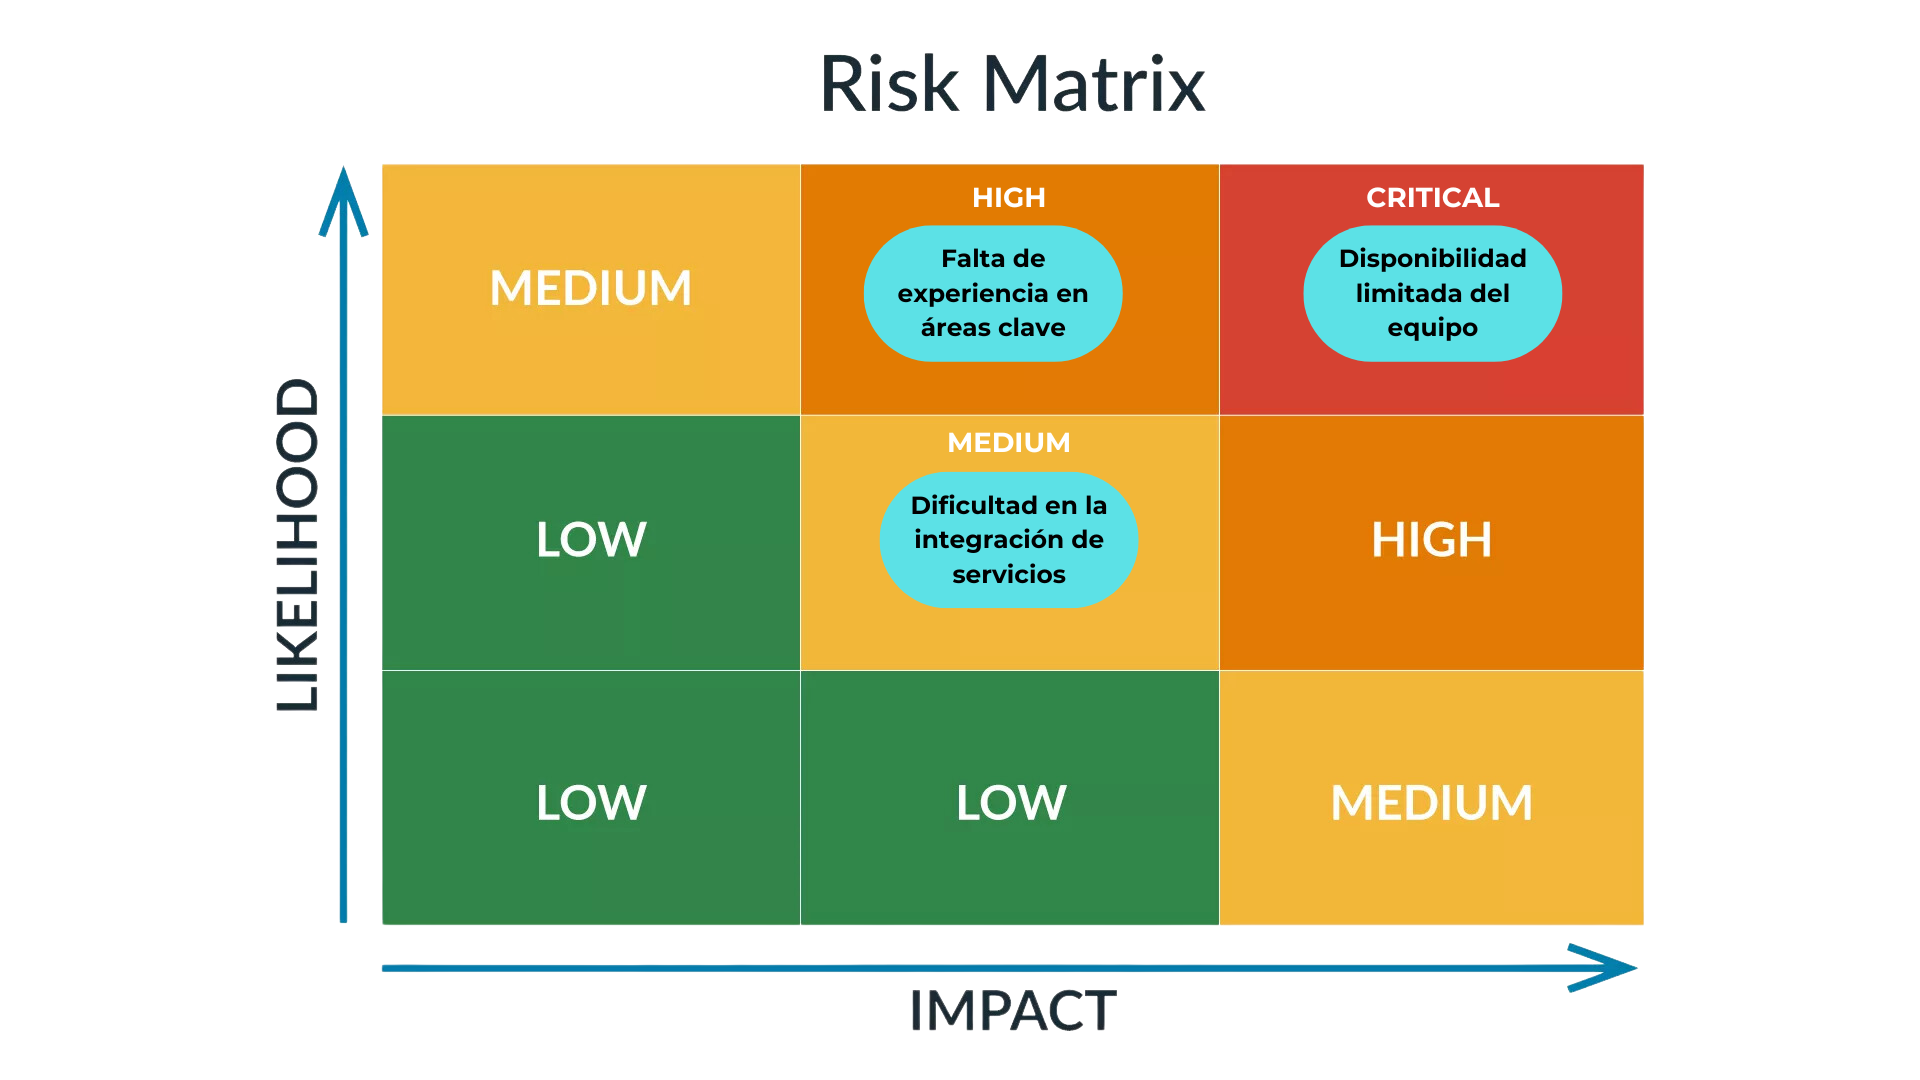
\includegraphics[width=\textwidth]{../imgs/proyecto.png}
\end{figure}

\begin{itemize}
    \item \textbf{Disponibilidad limitada del equipo} (Probabilidad Alta, Impacto Alto): Este riesgo se encuentra en el cuadrante \textbf{Crítico}.
    \item \textbf{Falta de experiencia en áreas clave} (Probabilidad Alta, Impacto Medio): Clasificado como \textbf{Alto}, este riesgo necesita medidas de mitigación, como capacitación o apoyo adicional.
    \item \textbf{Dificultad en la integración de servicios} (Probablidad Media, Impacto Medio): También clasificado como \textbf{Medio}, este riesgo afecta principalmente la fase de pruebas.
\end{itemize}

\begin{figure}[!ht]
    \centering
    \caption{Matriz de Riesgos del Producto}
    \label{fig:product_risk_matrix}
    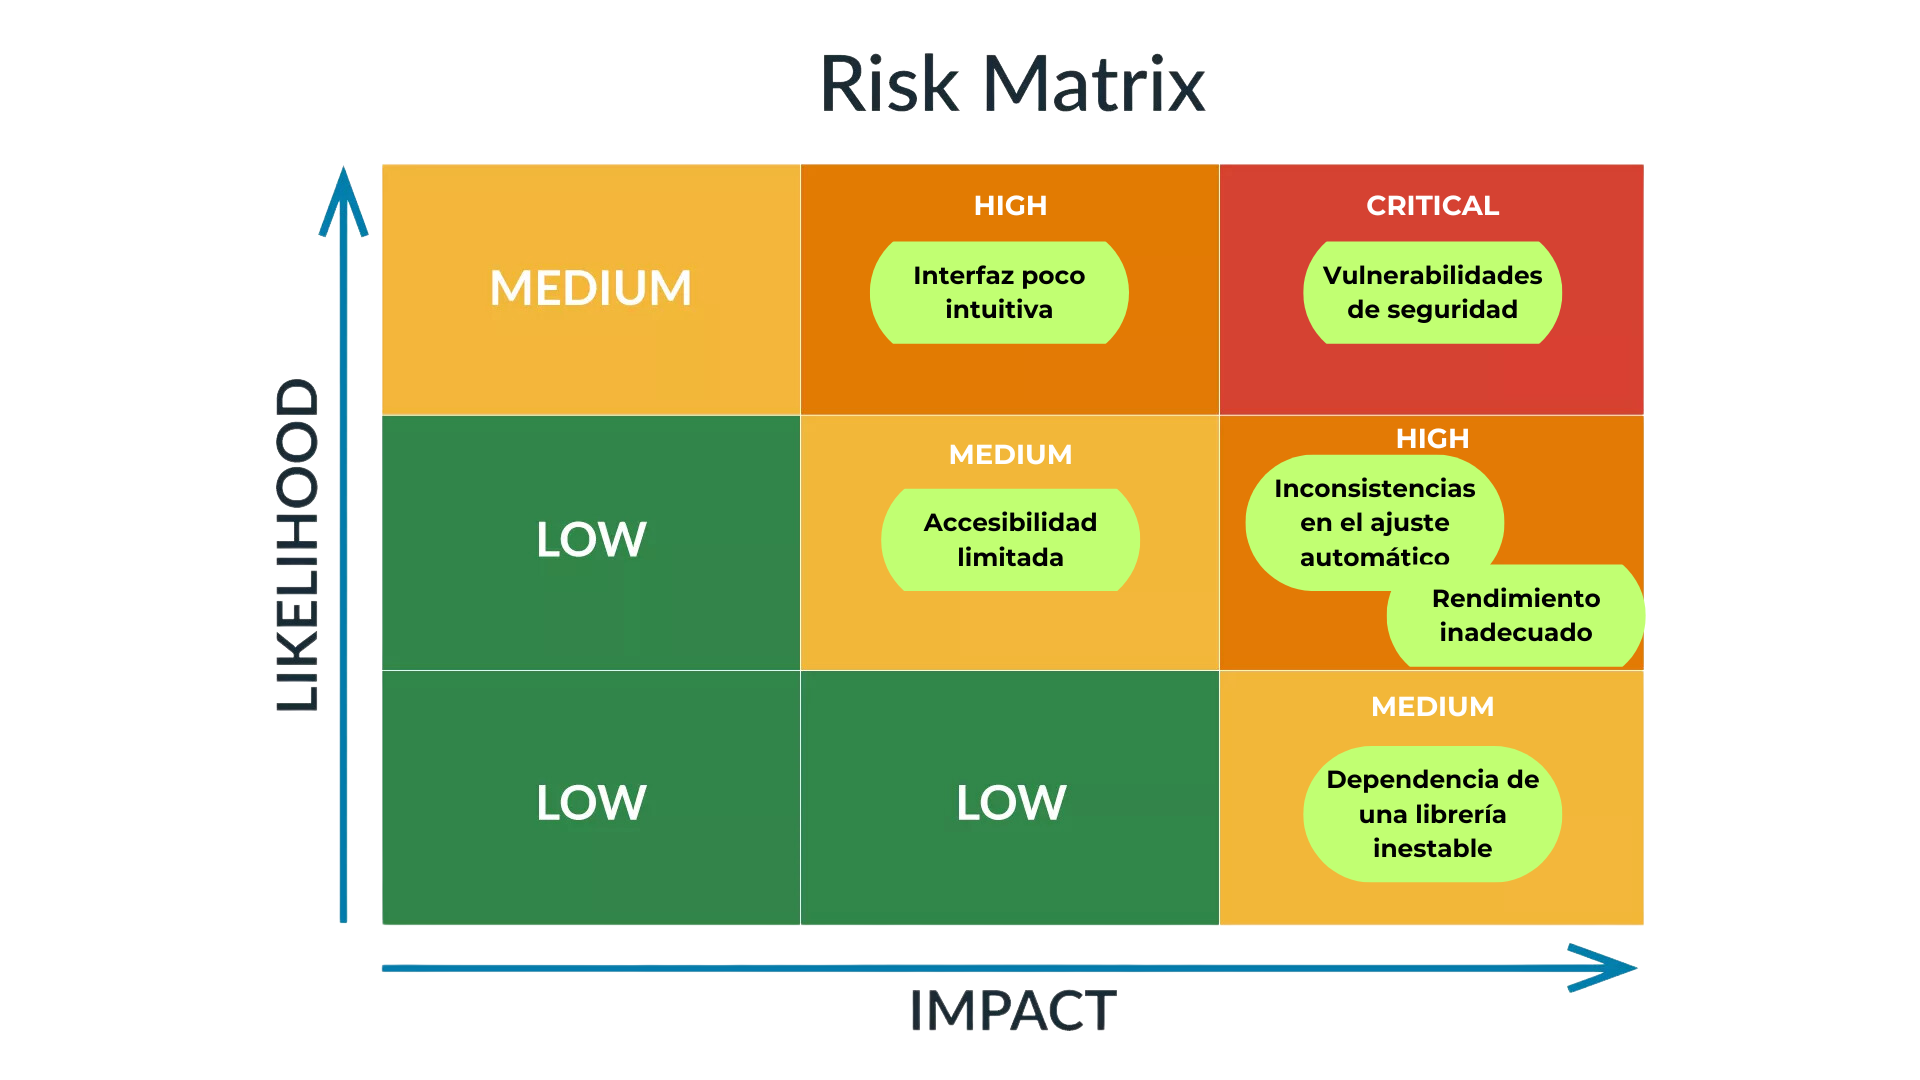
\includegraphics[width=\textwidth]{../imgs/producto.png}
\end{figure}

\begin{itemize}
    \item \textbf{Inconsistencias en el ajuste automático} y \textbf{Rendimiento inadecuado} (Probabilidad Media, Impacto Alto): Son riesgos \textbf{Altos}, recomendando acciones de mitigación urgentes para optimizar estas funcionalidades.
    \item \textbf{Vulnerabilidades de seguridad} (Probabilidad Alta, Impacto Alto): Se debe revisar la seguridad para proteger los datos de usuario.
    \item \textbf{Accesibilidad limitada} (Probabilidad Media, Impacto Medio): Clasificado como \textbf{Medio}, este riesgo requiere mejoras en la accesibilidad del editor.
    \item \textbf{Dependencia de una librería inestable} (Probabilidad Baja, Impacto Alto): Aunque la probabilidad es baja, el impacto es alto, lo que sugiere la necesidad de monitorear y actualizar la librería con precaución.
    \item \textbf{Interfaz y experiencia de usuario deficiente} (Probabilidad Alta, Impacto Medio): Clasificado como \textbf{Alto}, este riesgo requiere mejoras en la usabilidad y accesibilidad del editor.
\end{itemize}

\section{\large Presupuesto y Cronograma}
La estimación final es 32 horas-persona con un error estándar de aproximadamente 5.33 horas-persona. Esto significa que el esfuerzo estimado es de 32 horas-persona, pero podría variar en un rango de \(\pm 5.33\) horas debido a posibles incertidumbres. En base a esta estimación, se ha elaborado un cronograma detallado para el proyecto, que se muestra en la \hyperref[fig:cronograma]{Figura 3}.

\begin{figure}[!ht]
    \centering
    \caption{Cronograma del Proyecto: Diagrama de Gantt}
    \label{fig:cronograma}
    \begin{ganttchart}[
        hgrid,
        vgrid,
        time slot format=isodate,
        time slot unit=day
    ]{2024-10-15}{2024-10-28}
    
    % Define time labels
    \gantttitlecalendar{year, month=name, day} \\
    
    % Define tasks
    \ganttbar{Desarrollo del Plan de Pruebas}{2024-10-15}{2024-10-17} \\
    \ganttbar{Diseño y Creación de Test Cases}{2024-10-18}{2024-10-21} \\
    \ganttbar{Ejecución de Pruebas}{2024-10-22}{2024-10-24} \\
    \ganttbar{Análisis y Documentación de Defectos}{2024-10-25}{2024-10-26} \\
    \ganttbar{Creación del Informe Final}{2024-10-27}{2024-10-28} \\
    
    % Dependencies
    \ganttlink{elem0}{elem1}
    \ganttlink{elem1}{elem2}
    \ganttlink{elem2}{elem3}
    \ganttlink{elem3}{elem4}
    
    \end{ganttchart}
\end{figure}

\clearpage
\section{\large Enfoque de Prueba}

\noindent El enfoque de prueba para el editor \textit{Northwest} se centra en validar tanto los aspectos funcionales como no funcionales del sistema, asegurando que cumpla con los requisitos definidos y proporcione una experiencia de usuario satisfactoria.

\subsection{Niveles de Prueba}
Para asegurar la calidad del sistema, se realizarán pruebas en los siguientes niveles:
\begin{itemize}
    \item \textbf{Pruebas de Componentes}: Cada funcionalidad clave (como la creación de grafos, generación de matrices, y opciones de optimización) se probará de manera aislada para verificar su correcto funcionamiento.
    \item \textbf{Pruebas de Integración}: Validar la interacción entre componentes, especialmente entre la interfaz y los servicios backend, para asegurar que los datos fluyan correctamente.
    \item \textbf{Pruebas de Sistema}: Se evaluará la funcionalidad completa del editor, considerando la ejecución fluida de los procesos de prueba, generación de soluciones de optimización, y verificación de resultados.
\end{itemize}

\subsection{Tipos de Prueba}

\noindent En este proyecto, se implementarán diferentes tipos de prueba para asegurar una validación integral del editor \textit{Northwest}, abarcando tanto la funcionalidad como la experiencia de usuario.

\begin{itemize}
    \item \textbf{Pruebas Funcionales}: Estas pruebas aseguran que cada funcionalidad del editor cumpla con los requisitos establecidos, validando que el sistema se comporte como se espera en escenarios específicos. Las pruebas funcionales incluyen:
    \begin{itemize}
        \item \textbf{Validación de Creación y Visualización de Grafos}: Verifica que los grafos se creen correctamente con nodos y conexiones, y se visualicen de manera clara e intuitiva en la interfaz.
        \item \textbf{Carga y Descarga de Archivos}: Asegura que los grafos puedan ser guardados y recuperados sin pérdida de datos ni errores.
        \item \textbf{Generación de Matrices de Adyacencia y Costos}: Comprueba que el editor construya matrices precisas basadas en las conexiones y valores de los nodos.
        \item \textbf{Optimización de Soluciones}: Valida que el editor produzca soluciones correctas para los criterios de maximización y minimización.
    \end{itemize}

    \item \textbf{Pruebas No Funcionales}: Estas pruebas evalúan los aspectos que afectan la experiencia del usuario y el rendimiento del editor, asegurando que el sistema sea accesible, fácil de usar y responda adecuadamente bajo carga. Las pruebas no funcionales incluyen:
    \begin{itemize}
        \item \textbf{Pruebas de Usabilidad}: Basadas en las heurísticas de Nielsen, estas pruebas aseguran que la interfaz sea intuitiva y satisfactoria para el usuario.
        \item \textbf{Pruebas de Accesibilidad}: Verifican el cumplimiento de estándares básicos de accesibilidad, asegurando que el editor sea utilizable por personas con distintas capacidades.
        \item \textbf{Pruebas de Rendimiento}: Evaluarán, de manera específica, la capacidad de respuesta del sistema con grafos de tamaño y complejidad moderados, para asegurar que funcione correctamente bajo carga estándar.
    \end{itemize}

    \item \textbf{Pruebas de Caja Negra}: Estas pruebas se centran en validar el comportamiento del sistema sin analizar su lógica interna. Se utilizan para confirmar que las entradas proporcionadas generan las salidas esperadas, asegurando que el sistema cumpla con los requisitos funcionales sin considerar cómo se alcanzan los resultados. Son especialmente útiles para probar funcionalidades clave del editor como:
    \begin{itemize}
        \item \textbf{Validación de Resultados de Generación de Matrices}: La prueba introduce valores de entrada específicos (por ejemplo, conexiones y pesos) y verifica que el sistema genere correctamente matrices de adyacencia y de costos sin necesidad de analizar el código interno.
        \item \textbf{Optimización de Soluciones}: Introduce datos de oferta y demanda para evaluar si el sistema produce soluciones correctas (maximización o minimización), basándose únicamente en las salidas obtenidas.
        \item \textbf{Pruebas de Interfaz de Usuario}: Evalúa la funcionalidad de la interfaz para asegurarse de que los usuarios puedan crear grafos, visualizar matrices y obtener resultados sin errores visibles, abordando cualquier posible problema de interacción con el usuario.
    \end{itemize}
\end{itemize}



\subsection{Técnicas de Prueba}

\noindent Las técnicas de prueba aplicadas en este proyecto incluyen una combinación de técnicas de caja negra, caja blanca y herramientas específicas para la usabilidad y accesibilidad, para garantizar una validación exhaustiva del editor \textit{Northwest}.

\begin{itemize}
    \item \textbf{Técnicas de Caja Negra}:
    \begin{itemize}
        \item \textbf{Pruebas de Equivalencia de Clases}: Se utilizará para validar que el sistema maneja adecuadamente diferentes categorías de entrada (por ejemplo, valores válidos e inválidos en campos como oferta y demanda), agrupando los datos en clases de equivalencia. Esta técnica permite reducir el número de casos de prueba necesarios al probar solo una entrada representativa por clase.
    \end{itemize}

    \item \textbf{Técnicas para Usabilidad y Accesibilidad}:
    \begin{itemize}
        \item \textbf{Pruebas Basadas en Listas de Verificación (Checklists)}: Enfocadas en usabilidad, estas pruebas se basarán en listas de verificación construidas a partir de heurísticas de usabilidad de Nielsen para evaluar la facilidad de uso de la interfaz. La lista incluirá aspectos como claridad de la interfaz, accesibilidad de los elementos y consistencia en el diseño.
        \item \textbf{Pruebas de Accesibilidad con Axe DevTools}: Para verificar el cumplimiento de criterios de accesibilidad, se empleará la herramienta Axe DevTools, que permite realizar pruebas automáticas de accesibilidad en la interfaz y detectar posibles problemas, como bajo contraste de colores, falta de etiquetas en elementos interactivos y problemas de navegabilidad. Los resultados obtenidos con Axe DevTools se documentarán en el reporte de accesibilidad, asegurando que el sistema cumpla con estándares básicos de accesibilidad.
    \end{itemize}
\end{itemize}


\subsection{Criterios de Entrada y Salida}
\begin{itemize}
    \item \textbf{Criterios de Entrada}: Las pruebas estarán listas para ejecutarse cuando:
    \begin{itemize}
        \item Todos los servicios de backend estén configurados y ejecutándose en Docker.
        \item El entorno de frontend esté disponible, ya sea ejecutándose en Docker o localmente mediante el comando \texttt{npm run dev}.
        \item El proyecto esté en la rama \texttt{develop} para garantizar la estabilidad del entorno de pruebas.
        \item Todos los requisitos de datos de prueba estén definidos, incluyendo configuraciones específicas para nodos, matrices y otros parámetros requeridos.
        \item La interfaz de usuario y los servicios backend estén disponibles y funcionando correctamente.
    \end{itemize}
    
    \item \textbf{Criterios de Salida}: Las pruebas se considerarán finalizadas cuando:
    \begin{itemize}
        \item Se hayan ejecutado al menos cinco Test Cases definidos y se hayan documentado sus resultados y observaciones.
        \item Todos los criterios de éxito para alcanzar el nivel \texttt{AA} en la normativa WCAG de accesibilidad hayan sido evaluados y cumplidos.
        \item Se haya completado el checklist de usabilidad basado en las heurísticas de Nielsen, asegurando una experiencia de usuario óptima.
        \item Se haya finalizado el análisis de defectos encontrados y todos los hallazgos estén documentados en el informe de resultados.
        \item Todas las métricas definidas se hayan recopilado y se haya generado el dashboard de métricas para el análisis de resultados.
    \end{itemize}
\end{itemize}

\subsection{Independencia de las Pruebas}
Dado que el equipo de desarrollo participa también en el proceso de pruebas, las pruebas no serán completamente independientes. En este caso, Oscar Campohermoso Berdeja, quien participó en el desarrollo, también asume los roles de gestión y ejecución de pruebas. Para mitigar posibles conflictos de interés, se establecerán procedimientos claros para la documentación y revisión de resultados, asegurando que las pruebas sean objetivas y confiables.

\subsection{Métricas a Ser Recopiladas}
Durante la ejecución de las pruebas, se recopilarán las siguientes métricas:
\begin{itemize}
    \item \textbf{Número de Test Cases ejecutados} (totales, exitosos, fallidos).
    \item \textbf{Tasa de éxito de Test Cases} (porcentaje de pruebas exitosas).
    \item \textbf{Número de defectos identificados y categorizados} (funcionalidad, usabilidad, accesibilidad).
    \item \textbf{Tiempo total de ejecución de pruebas}, para estimar esfuerzos futuros.
\end{itemize}

\subsection{Requisitos de Datos de Prueba}
Los datos de prueba deben cubrir diferentes configuraciones de oferta y demanda, incluyendo:
\begin{itemize}
    \item Casos de oferta y demanda balanceados y no balanceados para verificar el ajuste automático del sistema.
    \item Configuraciones de matriz de costos con diferentes rangos de valores para probar maximización y minimización.
    \item Valores de entrada válidos e inválidos para evaluar la interfaz y los mensajes de error en el formulario de entrada.
\end{itemize}

\subsection{Requisitos del Entorno de Prueba}
El entorno de prueba se configurará utilizando Docker para asegurar una ejecución estable, aislada y reproducible de los servicios necesarios. Esto permite que el entorno sea fácilmente replicable y minimiza las variaciones en el comportamiento de las pruebas. Los servicios necesarios en el entorno de prueba incluyen:

\begin{itemize}
    \item \textbf{Backend implementado en FastAPI}: Este servicio maneja las solicitudes de optimización de transporte y debe estar configurado para responder a peticiones de la interfaz y los cálculos de matrices, asegurando un procesamiento eficiente y consistente de datos.
    \item \textbf{Servicios de almacenamiento}: Configurados para gestionar y almacenar archivos de configuración en formato JSON. Estos servicios garantizan la persistencia de datos y permiten la carga y recuperación de grafos y matrices sin pérdida de información.
    \item \textbf{Frontend desarrollado en Vue.js}: La interfaz gráfica del editor, desarrollada en Vue.js, permite la interacción del usuario con los elementos del editor. El frontend puede ejecutarse en Docker o de manera local, asegurando accesibilidad a todas las funcionalidades requeridas para la prueba.
\end{itemize}

Además, para asegurar la integridad del entorno, todos los servicios deben estar conectados mediante una red interna en Docker, permitiendo una comunicación fluida y segura entre los contenedores. Esta configuración facilitará la ejecución de pruebas automáticas y manuales en un entorno controlado, simulado y con condiciones similares a las de producción.



\newpage
% Referencias
\renewcommand\refname{\large\textbf{Referencias}}
\bibliographystyle{apacite}
\bibliography{mibibliografia}
\cite{nielsen1994}
\cite{dennis2015}
\cite{gregory2023}

\clearpage
\section{\large Anexos}
\subsection{Anexo A: Historias de Usuario}
\begin{table}[!ht]
    \centering
    \caption{Historia de Usuario HU006-GraphEditor}
    \label{tab:HU006-GraphEditor}
    \userstory{HU006-GraphEditor}{usuario de la aplicación}{poder agregar nodos, aristas y editar sus valores,}{poder construir y modificar gráficos de manera interactiva y visual.}{https://github.com/go-to-hell/proyecto-grafos-front/issues/50}
\end{table}

\begin{table}[!ht]
    \centering
    \caption{Historia de Usuario HU007-AdjacentMatrix}
    \label{tab:HU007-AdjacentMatrix}
    \userstory{HU007-AdjacentMatrix}{usuario de la aplicación}{obtener la matriz de adyacencia del grafo generado,}{poder visualizar las conexiones entre los nodos de forma estructurada y utilizar esta información posteriormente.}{https://github.com/go-to-hell/proyecto-grafos-front/issues/51}
\end{table}

\begin{table}[!ht]
    \centering
    \caption{Historia de Usuario HU008-FileManagement}
    \label{tab:HU008-FileManagement}
    \userstory{HU008-FileManagement}{usuario de la aplicación}{poder guardar el grafo realizado en formato JSON,}{cargarlo posteriormente y abrirlo en el mismo estado en el que lo dejé, conservando todos los nodos, aristas y configuraciones.}{https://github.com/go-to-hell/proyecto-grafos-front/issues/52}
\end{table}

\begin{table}[!ht]
    \centering
    \caption{Historia de Usuario HU009-NorthWest-01}
    \label{tab:HU009-NorthWest-01}
    \userstory{HU009-NorthWest-01}{usuario del sistema}{que la matriz de costos se genere automáticamente al crear nodos y conexiones,}{asegurarme de que los valores de los pesos reflejan correctamente las relaciones entre puntos de suministro y demanda.}{https://github.com/go-to-hell/proyecto-grafos-front/issues/53}
\end{table}

\begin{table}[!ht]
    \centering
    \caption{Historia de Usuario HU010-NorthWest-02}
    \label{tab:HU010-NorthWest-02}
    \userstory{HU010-NorthWest-02}{usuario del sistema}{manejar desequilibrios entre oferta y demanda, validando los campos obligatorios en el formulario de entrada,}{asegurarme de que se ajusten las soluciones automáticamente, evitando errores en el cálculo del transporte, y que pueda ingresar mis datos sin problemas, recibiendo retroalimentación clara en caso de errores.}{https://github.com/go-to-hell/proyecto-grafos-front/issues/54}
\end{table}

\begin{table}[!ht]
    \centering
    \caption{Historia de Usuario HU011-NorthWest-03}
    \label{tab:HU011-NorthWest-03}
    \userstory{HU011-NorthWest-03}{usuario del sistema}{generar soluciones válidas para las diferentes configuraciones que me da el sistema,}{poder confiar en la validez de los resultados y obtener diferentes resultados basados en el criterio de optimización que elija.}{https://github.com/go-to-hell/proyecto-grafos-front/issues/55}
\end{table}

\clearpage
\subsection{Anexo B: Diagramas de Flujo y Arquitectura}
\begin{figure}[H]
    \centering
    \caption{Diagrama de Flujo de Proceso para el Editor Northwest} \label{tab:flowchart}
    \begin{tikzpicture}[node distance=2cm, every node/.style={rounded corners, draw, align=center, minimum width=2.5cm, minimum height=1cm}]
    
        % Nodes
        \node (start) [fill=green!20] {Inicio};
        \node (createGraph) [below of=start, fill=blue!20] {Crear Grafo};
        \node (editGraph) [below of=createGraph, trapezium, trapezium left angle=70, trapezium right angle=110, fill=blue!10] {Editar nombre de Nodos \\ y agregar pesos a las Aristas};
        \node (saveProgress1) [right of=editGraph, xshift=5cm, trapezium, trapezium left angle=70, trapezium right angle=110, fill=yellow!10] {Guardar Avance};
        \node (generateAdjMatrix) [below of=editGraph, fill=blue!20] {Generar Matriz \\ de Adyacencia};
        \node (saveProgress2) [right of=generateAdjMatrix, xshift=5cm, trapezium, trapezium left angle=70, trapezium right angle=110, fill=yellow!10] {Guardar Avance};
        \node (generateCostMatrix) [below of=generateAdjMatrix, fill=blue!20] {Generar Matriz \\ de Costos};
        \node (fillDemandSupply) [below of=generateCostMatrix, trapezium, trapezium left angle=70, trapezium right angle=110, fill=blue!10] {Llenar datos de Demanda \\ y Oferta};
        \node (optimize) [below of=fillDemandSupply, diamond, aspect=2, yshift=-1cm, fill=orange!10] {Optimización \\ de Soluciones};
        \node (minimize) [below of=optimize, xshift=-3cm, fill=blue!20] {Minimizar};
        \node (maximize) [below of=optimize, xshift=3cm, fill=blue!20] {Maximizar};
        \node (resultMinimize) [below of=minimize, fill=blue!10, trapezium, trapezium left angle=70, trapezium right angle=110] {Resultado \\ Esperado};
        \node (resultMaximize) [below of=maximize, fill=blue!10, trapezium, trapezium left angle=70, trapezium right angle=110] {Resultado \\ Esperado};
        \node (end) [fill=red!20, below of=optimize, yshift=-2cm] {Fin};
        
        % Arrows
        \draw[->] (start) -- (createGraph);
        \draw[->] (createGraph) -- (editGraph);
        \draw[->] (editGraph) -- (generateAdjMatrix);
        \draw[->] (editGraph) -- (saveProgress1);
        \draw[->] (generateAdjMatrix) -- (generateCostMatrix);
        \draw[->] (generateAdjMatrix) -- (saveProgress2);
        \draw[->] (generateCostMatrix) -- (fillDemandSupply);
        \draw[->] (fillDemandSupply) -- (optimize);
        \draw[->] (optimize) -- (minimize);
        \draw[->] (optimize) -- (maximize);
        \draw[->] (minimize) -- (resultMinimize);
        \draw[->] (maximize) -- (resultMaximize);
        \draw[->] (resultMinimize) -- (end);
        \draw[->] (resultMaximize) -- (end);
    \end{tikzpicture}
\end{figure}


\begin{figure}[H]
    \centering
    \caption{Diagrama de Flujo de Datos para el Editor Northwest} \label{tab:dataflow}
    \begin{tikzpicture}[node distance=2cm]

        % Define styles for each type of node
        \tikzstyle{data} = [rectangle, minimum width=2.8cm, minimum height=0.8cm, text centered, draw=black, fill=purple!20]
        \tikzstyle{process} = [rectangle, minimum width=3cm, minimum height=1cm, text centered, draw=black, fill=blue!20]
        \tikzstyle{io} = [rectangle, minimum width=2.5cm, minimum height=1cm, text centered, draw=black, fill=orange!20]
        \tikzstyle{output} = [rectangle, minimum width=3cm, minimum height=1cm, text centered, draw=black, fill=green!30]
        \tikzstyle{decision} = [diamond, minimum width=3cm, minimum height=1cm, text centered, draw=black, fill=yellow!20]
        
        % Define arrow style
        \tikzstyle{arrow} = [thick,->,>=stealth]
        
        % Nodes
        \node (input) [io] {Entrada de Grafo};
        \node (graphData) [data, below of=input] {Datos de Grafo};
   
        
        % "Seleccionar Acción" se convierte en un nodo que muestra las posibles opciones
        \node (action) [process, below of=graphData, yshift=-0.5cm] {Definición de Datos};
        
        % Nodos de acciones en paralelo
        \node (adjMatrix) [process, below left of=action, xshift=-5cm, yshift=-1.5cm] {Generar Matriz de Adyacencia};
        \node (costMatrix) [process, below right of=action, xshift=5cm, yshift=-1.5cm] {Generar Matriz de Costos};
        \node (saveJson) [io, below of=action, yshift=-1cm] {Guardar Datos en JSON};
        
        % Conexión de las matrices y la optimización
        \node (saveAdjMatrix) [io, below of=adjMatrix, yshift=-1cm] {Guardar Datos en JSON};
        \node (optimize) [process, below of=costMatrix, yshift=-1cm] {Proceso de Datos};
        \node (output) [output, below of=optimize, yshift=-0.5cm] {Solución Optimizada};
        
        % Arrows
        \draw [arrow] (input) -- (graphData);
        \draw [arrow] (graphData) -- (action);
        
        % Opciones disponibles después de "Acciones Disponibles"
        \draw [arrow] (action) -- (adjMatrix);
        \draw [arrow] (action) -- (costMatrix);
        \draw [arrow] (action) -- (saveJson);
        
        % Continuación de flujos
        \draw [arrow] (adjMatrix) -- (saveAdjMatrix);
        \draw [arrow] (costMatrix) -- (optimize);
        \draw [arrow] (optimize) -- (output);

    \end{tikzpicture}
\end{figure}

\begin{figure}[H]
    \centering
    \label{fig:architecture}
    \caption{Arquitectura del sistema y sus interacciones principales}
    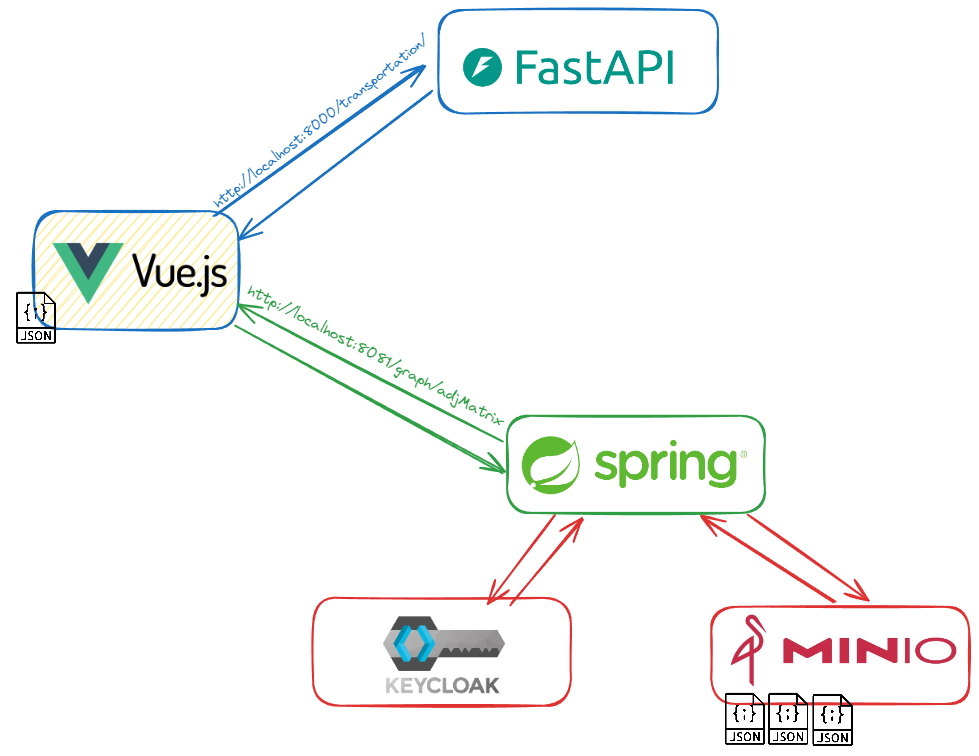
\includegraphics[width=\textwidth]{../imgs/architecture-2024-03-18-2220.png}
\end{figure}

\clearpage
\subsection{Anexo C: Plantillas del Reporte de Defectos}

\begin{longtable}{|p{5cm}|p{10cm}|}
    \caption{Plantilla de Reporte de Defectos} \label{tab:reporte_defectos} \\
    \hline
    \textbf{Test Case Reference} & \\ \hline
    \textbf{ID} & \\ \hline
    \textbf{Title} & \\ \hline
    \textbf{Description} & \\ \hline
    \textbf{Steps to Reproduce} & 
    1. \newline
    2. \newline
    3. \\ \hline
    \textbf{Expected Result} & \\ \hline
    \textbf{Actual Result} & \\ \hline
    \textbf{Evidence} & \\ \hline
    \textbf{Severity} & \\ \hline
    \textbf{Priority} & \\ \hline
\end{longtable}

\begin{longtable}{|>{\raggedright\arraybackslash}p{10cm}|>{\centering\arraybackslash}p{3cm}|}
    \caption{Plantilla de Reporte de Usabilidad} \label{tab:reporte_usabilidad} \\
    \hline
    \textbf{Items} & \textbf{Evaluation} \\ \hline
    
    \textbf{1.- Visibilidad del estado del sistema} & \\ \hline
    ¿Cada parte de la interfaz comienza con un título que describa el contenido de la pantalla? & \\ \hline
    ¿El diseño de íconos y su estética es consistente en todo el sistema? & \\ \hline
    Cuando se selecciona un icono que está rodeado de otros iconos, ¿Se distingue claramente el ícono seleccionado? & \\ \hline
    Si se utilizan ventanas emergentes (pop-up) para mostrar mensajes de error, ¿Permiten esas ventanas que el usuario visualice el error en la interfaz cuando se despliegan? & \\ \hline
    ¿Hay algún tipo de feedback para cada acción u operación? & \\ \hline
    Luego de que el usuario completa una acción o serie de acciones, ¿El "feedback" del sistema indica que el siguiente grupo de acciones puede completarse? & \\ \hline
    El sistema provee algún tipo de feedback visual en menús o cajas de diálogo que indiquen qué opciones pueden seleccionarse. & \\ \hline
    El sistema provee algún tipo de feedback visual en menús o cajas de diálogo que indiquen en cuál de las posibles opciones se halla posicionado el cursor. & \\ \hline
    Si hay menús o caja de diálogo en donde pueden seleccionarse múltiples opciones, ¿El sistema provee algún tipo de "feedback" visual que indique cuáles son las opciones ya seleccionadas? & \\ \hline
    ¿El sitio web entrega información corporativa de la organización? & \\ \hline
    Si existen demoras mayores a 15 segundos en las respuestas del sistema, ¿El usuario es informado del progreso en la concreción de la respuesta? & \\ \hline
    ¿Informa datos relevantes para quien no "navega" (Ej: Horas de atención)? ¿Y para hacer consultas web o no web (Ej: números de teléfono)? & \\ \hline
    ¿Los tiempos de respuesta son apropiados para cada tarea? & \\ \hline
    Tiempo de escritura, movimiento del cursor o selección con el ratón: entre 0,5 y 1,5 milisegundos & \\ \hline
    Tareas más comunes: 2 a 4 segundos & \\ \hline
    Tareas complejas: 8 a 12 segundos & \\ \hline
    No son necesarios altos niveles de concentración y no es requerido retener información: 2 a 15 segundos & \\ \hline
    La terminología usada en los menús, ¿Es consistente con el dominio de conocimiento del usuario en relación a la tarea a realizar? & \\ \hline
    ¿El usuario conoce su ruta de ubicación? & \\ \hline
    
    \textbf{2.- Relación entre el sistema y el mundo real} & \\ \hline
    ¿Los íconos son concretos y familiares para el usuario? & \\ \hline
    ¿Los colores seleccionados corresponden a los valores esperados? & \\ \hline
    Cuando se ingresan datos en la pantalla, ¿La terminología utilizada para describir la tarea es familiar para los usuarios? & \\ \hline
    Cuando la pantalla incluye preguntas, ¿El lenguaje de esas preguntas es claro y conciso? & \\ \hline
    Las combinaciones de secuencias de letras o palabras extrañas o poco frecuentes, ¿Se evitan siempre que sea posible? & \\ \hline
    El sistema ingresa/elimina de manera automática los signos de pesos o dólar y decimal cuando se insertan valores monetarios. & \\ \hline
    ¿Se utilizan nombres unívocos y descriptivos en todo momento? & \\ \hline
    ¿Se hace uso de los rastreadores de progreso? & \\ \hline
    Los H1 están optimizados para SEO & \\ \hline
    
    \textbf{3.- Control y libertad  por parte del usuario} & \\ \hline
    En sistemas que permitan el uso de ventanas superpuestas ¿Es fácil reacomodar reubicar esas ventanas en la pantalla? & \\ \hline
    En sistemas que permitan el uso de ventanas superpuestas ¿Es fácil para los usuarios cambiar de una ventana a otra? & \\ \hline
    Cuándo una tarea efectuada por el usuario se completa ¿el sistema espera alguna señal del usuario antes de procesar la tarea? & \\ \hline
    ¿Se pregunta al usuario que confime acciones que tendrán consecuencias drásticas, negativas o destructivas? & \\ \hline
    ¿Existe una función para "deshacer" al nivel de cada acción simple, cada entrada de datos y cada grupo de acciones completadas? & \\ \hline
    ¿Los usuarios pueden cancelar aacciones en progreso? & \\ \hline
    ¿Los usuarios pueden reducir el tiempo de entrada de datos copiando y modificando datos existentes? & \\ \hline
    Los menús son anchos (muchos ítems), antes que profundos (muchos niveles) & \\ \hline
    Si el sistema posee menús de niveles múltiples ¿Existe algún mecanismo que permita a los usuarios regresar al menú previo? & \\ \hline
    Los usuarios pueden moverse hacia delante o hacia atrás entre las opciones de campos o cajas de dialogo. & \\ \hline
    Si el sistema utiliza una interfaz de preguntas y respuestas ¿Pueden los usuarios regresar a la pregunta anterior o saltear hacia delante una pregunta? & \\ \hline
    ¿Los usuarios pueden revertir sus acciones de manera sencilla? & \\ \hline
    Si el sistema permite a los usuarios revertir sus acciones , ¿Existe un mecanismo que permita "deshacer" varias acciones de manera simultánea?  & \\ \hline

    \textbf{4.- Consistencia y estándares} & \\ \hline
    El abuso de letras en mayúscula en la pantalla se ha evitado & \\ \hline
    No hay más de 12/20 tipos de íconos & \\ \hline
    Existe algún elemento visual que identifique la ventana activa & \\ \hline
    Cada ventana posee un título & \\ \hline
    ¿Es posible utilizar las barras de desplazamiento horizontal y vertical en cada ventana? & \\ \hline
    Si una opción de un menú es la de "salir" ¿Esta opción aparece como ultimo ítem en el menú? & \\ \hline
    ¿Los títulos de los menús están centrados o justificados a la izquierda? & \\ \hline
    Fuentes: hasta tres tipos como máximo & \\ \hline
    Hasta cuatro colores (usados ocacionalmente)  & \\ \hline
    Sonido: tonos suaves para dispositivos de retroalimentación ocacional y bruscos para condiciones críticas. & \\ \hline
    ¿Se provee una leyenda si los códigos de color son numeros o dificiles de interpretar?  & \\ \hline
    Se evitan los pares de colores espectralmente extremos y altamente  cromáticos & \\ \hline
    Los azules saturados no se utilizan para texto u otro elemento pequeño. & \\ \hline
    La información más importante esta above the fold (la parte del sitio que los usuarios ven primero) & \\ \hline
    ¿La estructura de la entrada de datos es  consistente entre las diferentes pantallas? & \\ \hline

    \textbf{5.- Prevención de errores} & \\ \hline
    ¿Las entradas de datos no son sensibles a mayúsculas siempre que sea posible? & \\ \hline
    Las pantallas para entrada de datos y cajas de diálogo indican el número de espacios en caracteres que estan disponibles para un campo & \\ \hline
    Los campos en las pantallas de entrada de datos y las cajas de diálogo ¿contienen valores por defecto cuando corresponden? & \\ \hline


    \textbf{6.- Reconocer antes que recordar} & \\ \hline
    ¿Las áreas de texto tienen "espacios de respiración" que las rodeen? & \\ \hline
    ¿Se ha utilizado el mismo color para agrupar elementos relacionados? & \\ \hline
    ¿Existe buen contraste de brillo y de color entre los colores usados para imágines y fondos? & \\ \hline
    Los colores suaves, brillantes y saturados se han utilizado para enfatizar datos, mientras que los colores oscuros, opacos y no saturados, han sido usados para des-enfatizar datos? & \\ \hline
    ¿Los ítems inactivos en un menú aprecen en gris o están omitidos? & \\ \hline

    \textbf{7.- Flexibilidad y eficiencia en el uso} & \\ \hline
    Los usuarios pueden reducir el tiempo de entrada de datos si se les permite copiar y pegar datos existentes. & \\ \hline
    Si las listas de menú son cortas (siete ítem o menos) ¿Pueden los usuarios seleccionar un ítem moviendo el cursor? & \\ \hline

    \textbf{8.- Diseño estético y minimalista} & \\ \hline
    Los íconos son visuamente distinguibles de acuerdo a su significado conceptual  & \\ \hline
    ¿Cada ícono esta resaltado con respecto a su fondo? & \\ \hline
    Cada pantalla de entrada de datos incluye un título simple, corto, claro y suficientemente distintivo. & \\ \hline
    Los títulos de los menús son breves pero lo suficientemente largos como para comunicar su contenido. & \\ \hline

    \textbf{9.- Ayuda a los usuarios a reconocer, diagnosticar y recuperarse de los errores} & \\ \hline
    ¿Los sonidos son utilizados para señalar errores? & \\ \hline
    Si se usan mensajes de error con humor ¿Son apropiados y respetuosos para la comunidad de usuarios? & \\ \hline
    ¿Los mensajes de error son gramaticalmente correctos? & \\ \hline
    ¿Los mensajes de error evitan el uso de signos de admiración? & \\ \hline
    Los mensajes de error evitan el uso de palabras violentas u hostiles & \\ \hline
    Si se detecta un error en un campo de entrada de datos ¿El sistema posiciona el cursor en ese campo o lo resalta de alguna manera? & \\ \hline
    ¿Los mensajes de error sugieren la causa del problema que lo has ha ocacionado? & \\ \hline
    ¿Los mensajes de error indican que acción debe realizar el usuario para corregir el error correspondiente? & \\ \hline

    \textbf{10.- Ayuda y documentación} & \\ \hline
    ¿Las instrucciones en linea se distnguen visualmente?  & \\ \hline
    Si las opciones de los menús son ambiguas ¿el sistema provee información aclaratoria adacional cuando un ítem es seleccionado? & \\ \hline
    ¿La función de ayuda del menú es visible? (Por ejemplo una tecla etiquetada AYUDA o un menú especial) & \\ \hline
    Navegación: la información es facíl de encontrar & \\ \hline
    ¿La información es exacta, completa y comprensible? ¿La información es relevante? & \\ \hline
    Tras haber accedido a la ayuda ¿Pueden los usuarios continuar con su trabajo desde donde ha sido interrumpido? & \\ \hline
    ¿Es fácil acceder y regresar del sistema de ayuda? & \\ \hline
\end{longtable}

\begin{longtable}{|p{3cm}|p{10cm}|}
    \caption{Plantilla de Reporte de Accesibilidad} \label{tab:reporte_accesibilidad} \\
    \hline
    \multicolumn{2}{|c|}{\textbf{WCAG 2.1 AA}} \\ \hline
    \textbf{Guideline} & \textbf{Description of Violation} \\ \hline
    \endfirsthead

    \hline
    \multicolumn{2}{|c|}{\textbf{WCAG 2.1 AA}} \\ \hline
    \textbf{Guideline} & \textbf{Description of Violation} \\ \hline
    \endhead

    1 &  \\ \hline
    2 &  \\ \hline
\end{longtable}


    
\clearpage
\subsection{Anexo D: Casos de Prueba}

\small % Slightly reduce the font size for better fit
\renewcommand{\arraystretch}{1.0} % Slightly reduce the space between rows
\setlength{\tabcolsep}{4pt} % Reduce space between columns

\begin{longtable}{|p{2cm}|p{3cm}|p{3cm}|p{3cm}|p{3cm}|}
  \caption{Caso de prueba 1} \label{tab:casos_prueba1} \\
  \hline
  \multicolumn{5}{|l|}{\textbf{USER STORY REFERENCE: HU009-NorthWest-01, HU006-GraphEditor}} \\ \hline
  \textbf{TEST CASE ID} & \textbf{TEST DATE} & \textbf{TEST DESCRIPTION} & \textbf{TEST CONDITIONS} & \textbf{SEVERITY} \\ \hline
  \endfirsthead
  \hline
  \textbf{STEP ID} & \textbf{STEP DESCRIPTION} & \textbf{TEST DATE} & \textbf{EXPECTED RESULTS} & \textbf{ACTUAL RESULTS} \\ \hline
  \endhead
  TC1-NW & 2024-10-17 & Comprobar que, al crear los nodos y las conexiones, se genera automáticamente la matriz con los valores correctos de los pesos. & El editor debe estar configurado correctamente. Los nodos de origen y destino deben poder ser creados y conectados sin errores. Los pesos asignados deben ser valores numéricos válidos y compatibles con el sistema. & ALTA \\ \hline
  \textbf{STEP ID} & \textbf{STEP DESCRIPTION} & \textbf{TEST DATE} & \textbf{EXPECTED RESULTS} & \textbf{ACTUAL RESULTS} \\ \hline
  S1-NW & Crear 3 nodos de origen y 3 nodos de destino en el editor. & 2024-10-17 & Los 6 nodos son creados correctamente sin errores. & \\ \hline
  S2-NW & Asignar conexiones entre ellos con pesos específicos para cada enlace. & 2024-10-17 & Las conexiones se establecen correctamente y los pesos asignados son visibles en la interfaz. & \\ \hline
  S3-NW & Abrir el formulario "Northwest" para ver la matriz generada. & 2024-10-17 & La matriz generada muestra los valores de los pesos correctamente, coincidiendo con los valores de las conexiones creadas. & \\ \hline
\end{longtable}


\begin{longtable}{|p{2cm}|p{3cm}|p{3cm}|p{3cm}|p{3cm}|}
    \caption{Caso de prueba 2} \label{tab:casos_prueba2} \\
    \hline
    \multicolumn{5}{|l|}{\textbf{USER STORY REFERENCE: HU009-NorthWest-01, HU010-NorthWest-02}} \\ \hline
    \textbf{TEST CASE ID} & \textbf{TEST DATE} & \textbf{TEST DESCRIPTION} & \textbf{TEST CONDITIONS} & \textbf{SEVERITY } \\ \hline
    \endfirsthead
    \hline
    \textbf{STEP ID} & \textbf{STEP DESCRIPTION} & \textbf{TEST DATE} & \textbf{EXPECTED RESULTS} & \textbf{ACTUAL RESULTS} \\ \hline
    \endhead
    TC2-NW & 2024-10-17 & Verificar el comportamiento del sistema cuando la suma de la oferta y la demanda no es igual. & El editor debe estar configurado correctamente. Los nodos de origen y destino deben poder ser creados y conectados sin errores. Los pesos asignados deben ser valores numéricos válidos y compatibles con El sistema. La oferta total debe ser mayor que  la demanda. & MEDIA                                                                                                     \\ \\ \hline
    \textbf{STEP ID} & \textbf{STEP DESCRIPTION} & \textbf{TEST DATE} & \textbf{EXPECTED RESULTS} & \textbf{ACTUAL RESULTS} \\ \hline
    S1-2-NW & Ingresar 100 unidades de oferta para los nodos de origen & 2024-10-17 & El sistema debe aceptar la cantidad de oferta sin mostrar errores. & \\ \hline
    S2-2-NW & Ingresar 80 unidades de demanda para los nodos de destino. & 2024-10-17 & El sistema debe aceptar la cantidad de demanda sin mostrar errores. & \\ \hline
    S3-2-NW & Ejecutar el cálculo utilizando el método de la esquina noroeste. & 2024-10-17 & El sistema debe detectar que la oferta y la demanda no están balanceadas y ajustar automáticamente la solución (por ejemplo, añadiendo un nodo ficticio) para resolver el problema de transporte sin errores. & \\ \hline
\end{longtable}


\begin{longtable}{|p{2cm}|p{3cm}|p{3cm}|p{3cm}|p{3cm}|}
    \caption{Caso de prueba 3} \label{tab:casos_prueba3} \\
    \hline
    \multicolumn{5}{|l|}{\textbf{USER STORY REFERENCE: HU010-NorthWest-02, HU010-NorthWest-03}} \\ \hline
    \textbf{TEST CASE ID} & \textbf{TEST DATE} & \textbf{TEST DESCRIPTION} & \textbf{TEST CONDITIONS} & \textbf{SEVERITY } \\ \hline
    \endfirsthead
    \hline
    \textbf{STEP ID} & \textbf{STEP DESCRIPTION} & \textbf{TEST DATE} & \textbf{EXPECTED RESULTS} & \textbf{ACTUAL RESULTS} \\ \hline
    \endhead
    TC3-NW & 2024-10-17 & Verificar que las opciones de maximizar y minimizar generen soluciones distintas. & El editor debe estar configurado correctamente, permitiendo crear y conectar nodos. Pesos numéricos válidos y matriz de costos conocida. & ALTA \\ \hline
    \textbf{STEP ID} & \textbf{STEP DESCRIPTION} & \textbf{TEST DATE} & \textbf{EXPECTED RESULTS} & \textbf{ACTUAL RESULTS} \\ \hline
    S1-3-NW & Configurar la matriz de costos. & 2024-10-17 & El sistema acepta la matriz de costos sin errores y la muestra correctamente. & \\ \hline
    S2-3-NW & Seleccionar maximización y calcular. & 2024-10-17 & El sistema calcula y muestra la solución sin errores. &  \\ \hline
    S3-3-NW & Verificar la solución en maximización. & 2024-10-17 & Solución visible y accesible en la interfaz. & \\ \hline
    S4-3-NW & Seleccionar minimización y calcular. & 2024-10-17 & El sistema calcula y muestra la solución sin errores. & \\ \hline
    S5-3-NW & Comparar ambas soluciones. & 2024-10-17 & \\ \hline
\end{longtable}

\begin{longtable}{|p{2cm}|p{3cm}|p{3cm}|p{3cm}|p{3cm}|}
    \caption{Caso de prueba 4} \label{tab:casos_prueba4} \\
    \hline
    \multicolumn{5}{|l|}{\textbf{USER STORY REFERENCE: HU009-NorthWest-01, HU010-NorthWest-03}} \\ \hline
    \textbf{TEST CASE ID} & \textbf{TEST DATE} & \textbf{TEST DESCRIPTION} & \textbf{TEST CONDITIONS} & \textbf{SEVERITY} \\ \hline

    \endfirsthead
    \hline
    \textbf{STEP ID} & \textbf{STEP DESCRIPTION} & \textbf{TEST DATE} & \textbf{EXPECTED RESULTS} & \textbf{ACTUAL RESULTS} \\ \hline
    \endhead
    TC4-NW & 2024-10-17 & Verificar que el sistema siempre genere una solución factible para diferentes configuraciones de oferta y demanda. & El editor debe estar configurado correctamente. Los nodos de origen y destino deben poder ser creados y conectados sin errores. Los pesos asignados deben ser valores numéricos válidos y compatibles con El sistema. Varias configuraciones de oferta y demanda, incluyendo configuraciones balanceadas y no balanceadas. & ALTA                                                                                           \\ \\ \hline
    \textbf{STEP ID} & \textbf{STEP DESCRIPTION} & \textbf{TEST DATE} & \textbf{EXPECTED RESULTS} & \textbf{ACTUAL RESULTS} \\ \hline
    S1-4-NW & Ingresar diferentes valores de oferta y demanda (balanceados y no balanceados). & 2024-10-17 & El sistema debe aceptar los valores de oferta y demanda sin errores, independientemente de si están balanceados. &  \\ \hline
    S2-4-NW & Ejecutar el cálculo del problema de transporte utilizando el módulo "Northwest". & 2024-10-17 & El sistema debe generar una solución válida y consistente, sin importar si la configuración de oferta y demanda está balanceada. & \\ \hline
\end{longtable}

\begin{longtable}{|p{2cm}|p{3cm}|p{3cm}|p{3cm}|p{3cm}|}
    \caption{Caso de prueba 5} \label{tab:casos_prueba5} \\
    \hline
    \multicolumn{5}{|l|}{\textbf{USER STORY REFERENCE: HU009-NorthWest-02}} \\ \hline
    \textbf{TEST CASE ID} & \textbf{TEST DATE} & \textbf{TEST DESCRIPTION} & \textbf{TEST CONDITIONS} & \textbf{SEVERITY} \\ \hline
    \endfirsthead
    \hline
    \textbf{STEP ID} & \textbf{STEP DESCRIPTION} & \textbf{TEST DATE} & \textbf{EXPECTED RESULTS} & \textbf{ACTUAL RESULTS} \\ \hline
    \endhead
    TC5-NW & 2024-10-17 & Asegurarse de que el formulario de entrada de datos sea intuitivo y que los campos obligatorios estén correctamente validados. & El editor debe estar configurado correctamente. Los nodos de origen y destino deben poder ser creados y conectados sin errores. Datos válidos e inválidos en el formulario de entrada, incluyendo campos vacíos y datos no numéricos en los campos de oferta y demanda. & ALTA \\ \hline
    \textbf{STEP ID} & \textbf{STEP DESCRIPTION} & \textbf{TEST DATE} & \textbf{EXPECTED RESULTS} & \textbf{ACTUAL RESULTS} \\ \hline
    S1-5-NW & Intentar enviar el formulario con algunos campos vacíos. & 2024-10-17 & El sistema debe mostrar mensajes de error específicos indicando que los campos obligatorios están vacíos. & \\ \hline
    S2-5-NW & Ingresar datos no numéricos en los campos de oferta y demanda y enviar el formulario. & 2024-10-17 & El sistema debe mostrar mensajes de error indicando que los valores en oferta y demanda deben ser numéricos. & \\ \hline
    S3-5-NW & Ingresar datos válidos en todos los campos y enviar el formulario, sin demanda y oferta. & 2024-10-17 & El sistema debe lanzar un mensaje de error porque los datos de demanda y oferta deberían ser obligatorios. & \\ \hline
\end{longtable}

\small % Slightly reduce the font size for better fit
\renewcommand{\arraystretch}{1.0} % Slightly reduce the space between rows
\setlength{\tabcolsep}{4pt} % Reduce space between columns

\begin{longtable}{|p{2cm}|p{3cm}|p{3cm}|p{3cm}|p{3cm}|}
    \caption{Caso de prueba 6} \label{tab:casos_prueba6} \\
    \hline
    \multicolumn{5}{|l|}{\textbf{USER STORY REFERENCE: HU006-GraphEditor}} \\ \hline
    \textbf{TEST CASE ID} & \textbf{TEST DATE} & \textbf{TEST DESCRIPTION} & \textbf{TEST CONDITIONS} & \textbf{SEVERITY} \\ \hline
    \endfirsthead
    \hline
    \textbf{STEP ID} & \textbf{STEP DESCRIPTION} & \textbf{TEST DATE} & \textbf{EXPECTED RESULTS} & \textbf{ACTUAL RESULTS} \\ \hline
    \endhead
    TC6-NW & 2024-10-17 & Verificar que el editor permita a los usuarios definir nodos y conexiones con pesos, y que los grafos se visualicen de forma intuitiva en la interfaz. & Configuración inicial del editor sin grafos; usuarios con capacidad de definir nodos y conexiones. & ALTA \\ \hline
    \textbf{STEP ID} & \textbf{STEP DESCRIPTION} & \textbf{TEST DATE} & \textbf{EXPECTED RESULTS} & \textbf{ACTUAL RESULTS} \\ \hline
    S1-6-NW & Definir un nodo en el editor. & 2024-10-17 & El nodo debe aparecer inmediatamente en la visualización gráfica del editor. & \\ \hline
    S2-6-NW & Ingresar datos válidos en todos los campos y enviar el formulario. & 2024-10-17 & La conexión debe visualizarse en el grafo en tiempo real, mostrando el peso asignado. & \\ \hline
    S3-6-NW & Intentar crear una conexión con datos inconsistentes (por ejemplo, un peso no numérico). & 2024-10-17 & El sistema debe notificar al usuario sobre la inconsistencia en la entrada de datos, previniendo errores en la creación del grafo. & \\ \hline
    S4-6-NW & Modificar la conexión o el nodo existente. & 2024-10-17 & La visualización del grafo debe actualizarse de inmediato para reflejar los cambios realizados. & \\ \hline
\end{longtable}

\small % Slightly reduce the font size for better fit
\renewcommand{\arraystretch}{1.0} % Slightly reduce the space between rows
\setlength{\tabcolsep}{4pt} % Reduce space between columns

\begin{longtable}{|p{2cm}|p{3cm}|p{3cm}|p{3cm}|p{3cm}|}
    \caption{Caso de prueba 7} \label{tab:casos_prueba7} \\
    \hline
    \multicolumn{5}{|l|}{\textbf{USER STORY REFERENCE: HU008-FileManagement}} \\ \hline
    \textbf{TEST CASE ID} & \textbf{TEST DATE} & \textbf{TEST DESCRIPTION} & \textbf{TEST CONDITIONS} & \textbf{SEVERITY} \\ \hline
    \endfirsthead
    \hline
    \textbf{STEP ID} & \textbf{STEP DESCRIPTION} & \textbf{TEST DATE} & \textbf{EXPECTED RESULTS} & \textbf{ACTUAL RESULTS} \\ \hline
    \endhead
    TC7-NW & 2024-10-17 & Verificar que el editor permita cargar grafos desde el computador en formato JSON y descargar los grafos creados, con notificaciones de éxito o error en las operaciones. & Grafo guardado en formato JSON en el computador; editor configurado para cargar y descargar grafos. & ALTA \\ \hline
    \textbf{STEP ID} & \textbf{STEP DESCRIPTION} & \textbf{TEST DATE} & \textbf{EXPECTED RESULTS} & \textbf{ACTUAL RESULTS} \\ \hline
    S1-7-NW & Cargar un archivo JSON de grafo desde el computador al editor. & 2024-10-17 & El grafo debe aparecer correctamente en el editor, conservando todos los nodos y conexiones, y el sistema debe notificar que la carga fue exitosa. & \\ \hline
    S2-7-NW & Intentar cargar un archivo JSON con datos incompletos o en formato incorrecto. & 2024-10-17 & El sistema debe mostrar un mensaje de error indicando el problema con el archivo, sin cargar datos incompletos en el editor. & \\ \hline
    S3-7-NW & Descargar el grafo actualmente visualizado en el editor en formato JSON. & 2024-10-17 & El archivo debe descargarse correctamente, conservando toda la información de nodos y conexiones, y el sistema debe notificar que la descarga fue exitosa. & \\ \hline
\end{longtable}


\end{document}